%
% File: chap03.tex
% Author:
% Description: Design and Implementations
%
\chapter{Design and Implementations}
\label{chap:D&I}

Begins a chapter. Example: When the beloved cellist (Christopher Walken - outstanding) of a world-renowned string quartet receives a life-changing diagnosis, the group's future suddenly hangs in the balance: suppressed emotions, competing egos and uncontrollable passions threaten to derail years of friendship and collaboration. Featuring a brilliant ensemble cast (including Philip Seymour Hoffman, Catherine Keener and Mark Ivanir as the three other quartet members), it is a fascinating look into the world of working musicians, and an elegant homage to chamber music and the cultural world of New York. The music, of course, is ravishing (the score is the work of regular David Lynch collaborator Angelo Badalamenti): A Late Quartet hits all the right notes.

\section{Methodology}
\label{sec:sec01}

\subsection{Work Flow}
\label{subsec:subsec01}

\subsection{Process}
\label{subsec:subsec02}

\subsection{Front-end Tools}
\label{subsec:subsec03}

\subsection{Back-end Tools}
\label{subsec:subsec04}

\subsection{Testing Tools}
\label{subsec:subsec05}

\section{Front-end Design and Implementations}
\label{sec:sec02}

\subsection{Early Stage-Virtual Hospital Africa(VHA)}
\label{subsec:subsec01}

During initial discussions with the client about their requirements, the client pointed out that the current website's Patient Intake page contained too many information fields, leading to poor user experience and even many testers abandoning the form midway during testing (Figure 3.1). Based on this situation, the client designed a second version of the multi-step form interface (Figure 3.2). The original form was split into separate pages (personal information, contact information, primary care, reason for visit), each with a progress indicator to guide users through the process.

During the programming and testing of the second version design, group members identified several issues that could potentially impact usability in actual interactions. We conducted internal team discussions and shared these issues with the client during our weekly design meetings. Ultimately, the client adopted our suggestions and finalized the third version design (Figure 3.3), with the following key improvements:

\begin{itemize}
    \item 1. Added a left-side navigation bar to enable non-linear navigation
\end{itemize}
The original design relied solely on the top progress bar, requiring users to complete steps in a fixed order. We suggested adding a modular navigation bar on the left side, allowing users to freely jump to any section for modifications, thereby enhancing their sense of control and flexibility \cite{nielsen1995}..

\begin{itemize}
    \item 2. Optimized field grouping and information hierarchy
\end{itemize}
We consolidated information such as name, gender, title, language, and national ID number into the “General” group and introduced a profile photo upload function on this page to add a patient profile photo capture/upload feature. This aligns the website's information layout with users' real-world information collection habits and aligns with the standard practice in hospital admission processes of “first collecting basic information and taking photos for record-keeping.” Additionally, once the avatar upload is complete, a preview will be displayed immediately, and the centralized presentation of related fields will allow users to quickly confirm the accuracy of key information in a unified area, ensuring visibility of the interaction process \cite{nielsen1995}..

\begin{itemize}
    \item 3. Unify navigation button layout
\end{itemize}
In the third version design, since we removed the top global navigation bar, users need clearer prompts for the next steps in the interface. Based on Nielsen's (1995) usability principles of “Visibility of system status” and “Match between system and the real world,” we replaced the bottom buttons with ‘Back’ and “Next” as alternative navigation methods, clearly indicating the user's forward and return paths. This design reduces users' sense of disorientation during task flows, enhances the predictability of operations, and increases the certainty of task completion.

Regarding the second group: The client's requirements primarily focused on the patient profile page, highlighting several shortcomings in the current interface regarding information presentation and user experience. These include lack of detailed patient identification methods and information, absence of quick access points, unclear information structure, absence of direct editing functions, low efficiency in switching between information modules, and insufficient visual hierarchy in the interface (Figure 3.4). In response to the client's requirements, we proposed several improvement suggestions, which were confirmed in subsequent meetings with the client, ultimately resulting in the design of the new version (Figure 3.5):

\begin{itemize}
    \item 1. Enhance the patient information card: Add a profile picture, gender/age tags, patient status, quick contact button, download patient report button, and last edit time to the patient information card. This not only avoids healthcare staff having to make additional clicks or page switches to confirm patient identity and status but also addresses the issue of being unable to perform common operations directly on the patient profile page, enabling quick identification and efficient management of patient information.
    \item 2. Expand the patient information module and optimize the information navigation structure: Introduce more patient information modules in the Patient Profile, unify the naming and order of the top tab bar, and add a secondary menu on the left side, dividing the information into modules such as General, Primary Care, Contacts, Biometrics, and Insurance. This modular structure enhances the completeness of the information, allowing users to efficiently obtain the required data on a single page and reducing the need for frequent page switching or scrolling to find information.
    \item 3. Switch to editable forms: Present personal information in structured fields that support direct editing. This simplifies the information maintenance process, reduces operational steps, and enhances the user experience.
\end{itemize}
The third group of customers' needs were mainly focused on the Vitals page, and they pointed out that the current interface had many shortcomings in terms of data input structure and interaction experience, mainly including: all vital signs items were stacked in a single list, with no clear distinction between required and optional fields, making it difficult for users to quickly identify which fields to fill in first; the order of the fields did not fully match the clinical data collection process, and some commonly used data items were not placed prominently enough; the page lacked step-by-step navigation or process guidance, and users might not be able to confirm their progress(Figure 3.6). After internal discussions, we proposed improvement suggestions for these issues and reached consensus with the client during meetings, ultimately finalizing the new version design (Figure 3.7):

\begin{itemize}
    \item 1. Grouped layout and priority adjustments
\end{itemize}
Vital sign information is divided into two main sections: “Required” and “Optional,” ensuring that healthcare professionals prioritize the collection of critical data; the field order is adjusted to better align with actual clinical data collection practices (e.g., first entering height, weight, temperature, blood pressure, and pulse rate, followed by optional items such as blood glucose, oxygen saturation, and respiratory rate). \cite{webform}.

\begin{itemize}
    \item 2. Optimized operational workflow
\end{itemize}
Added Back/Next navigation buttons at the bottom of the page to replace the original single “Continue” button, allowing users to more intuitively control the progress of form completion and avoid omissions due to skipping or accidental operations.

\begin{itemize}
    \item 3. Integration with patient information panel
\end{itemize}
Retained the patient profile summary and treatment timeline (Seeking Treatment) on the right side, ensuring that healthcare professionals can reference the patient's status and completed examination steps at any time during data entry.

These changes adhere to usability principles such as “Match between system and the real world,” “Visibility of system status,” and “Recognition rather than recall,” reducing cognitive load, improving data entry efficiency, and minimizing operational errors. \cite{nielsen1995}.

\begin{figure}[H]
    \centering
    \begin{minipage}{0.47\textwidth}
        \centering
        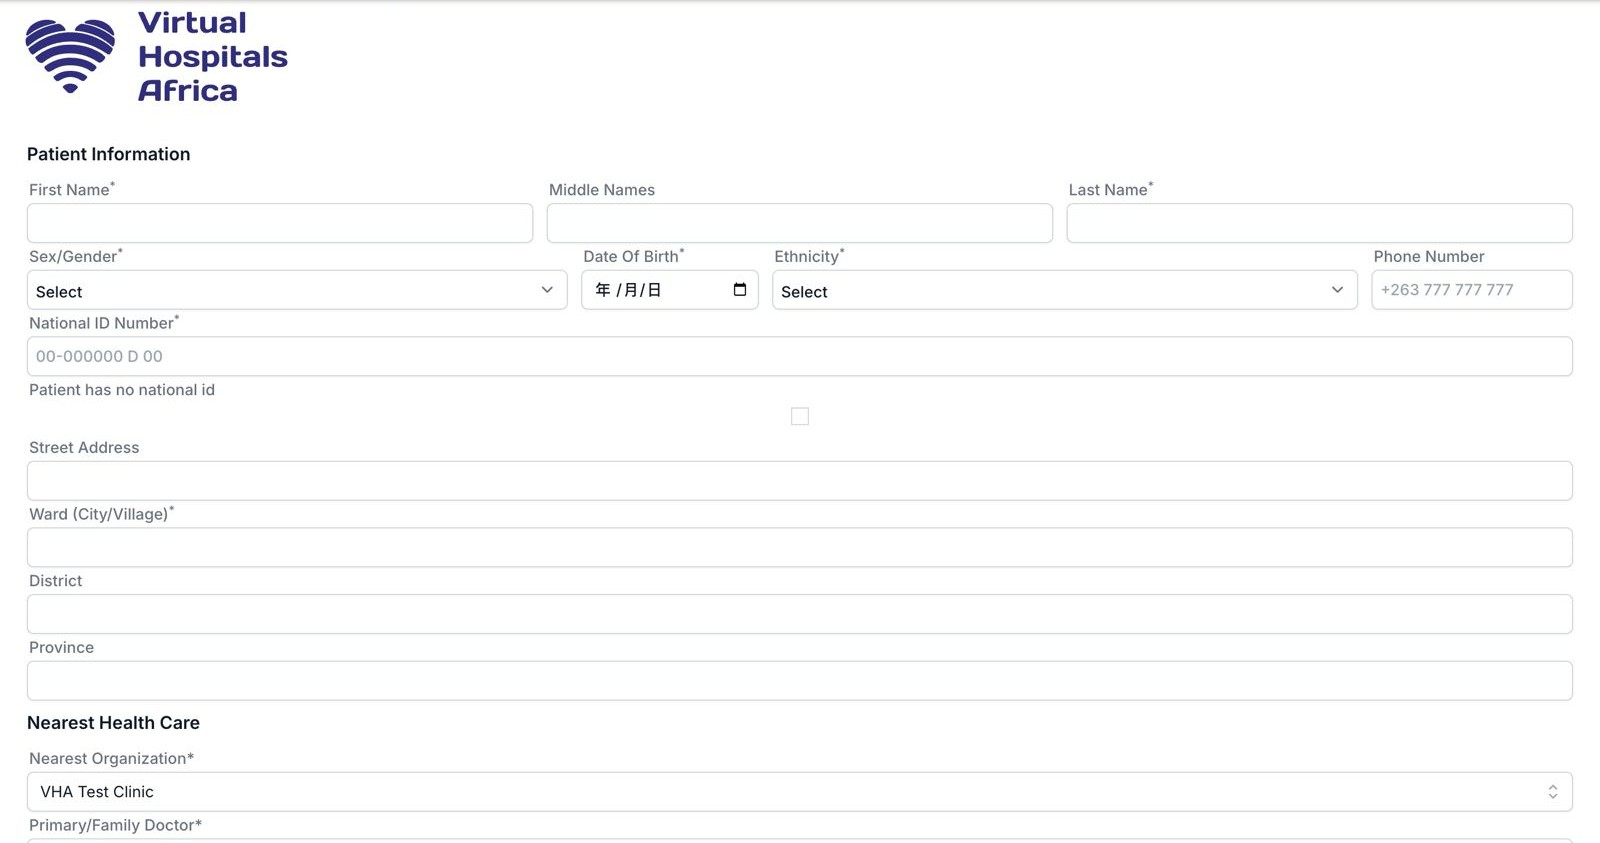
\includegraphics[width=\textwidth]{images/(VHA)-1.jpg}
        \caption{Patient Intake page – original version / user feedback context}
        \label{fig:design-1}
    \end{minipage}\hfill
    \begin{minipage}{0.47\textwidth}
        \centering
        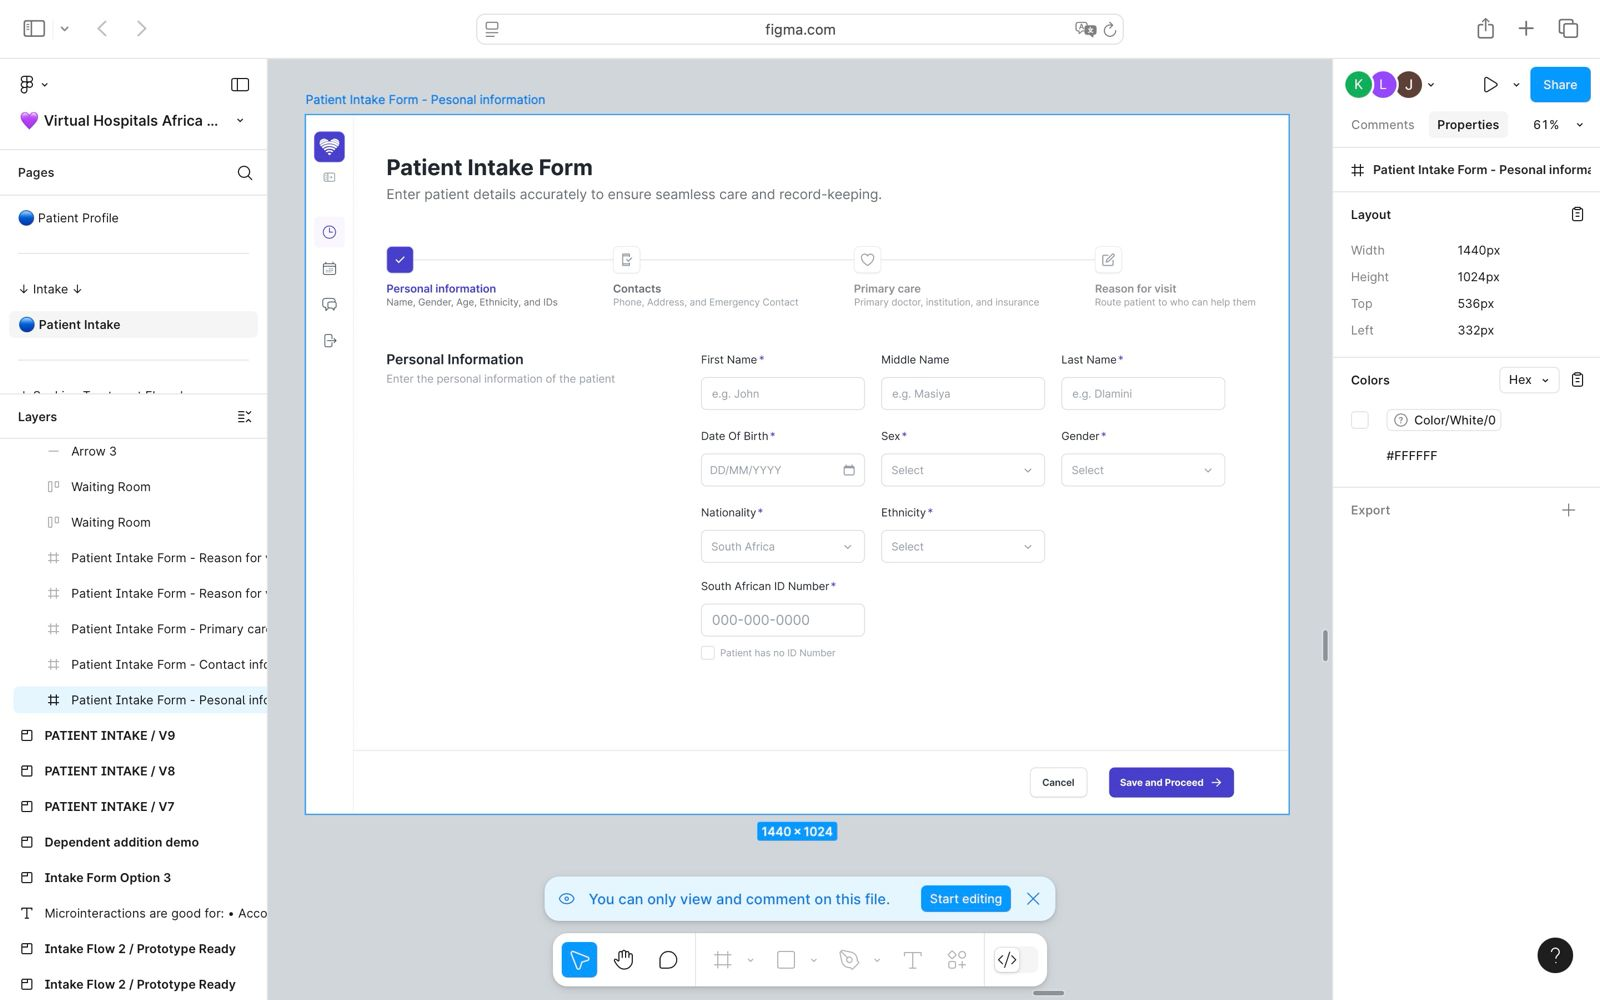
\includegraphics[width=\textwidth]{images/(VHA)-2.jpg}
        \caption{Second version multi-step form interface}
        \label{fig:design-2}
    \end{minipage}
\end{figure}
\begin{figure}[H]
    \centering
    \begin{minipage}{0.47\textwidth}
        \centering
        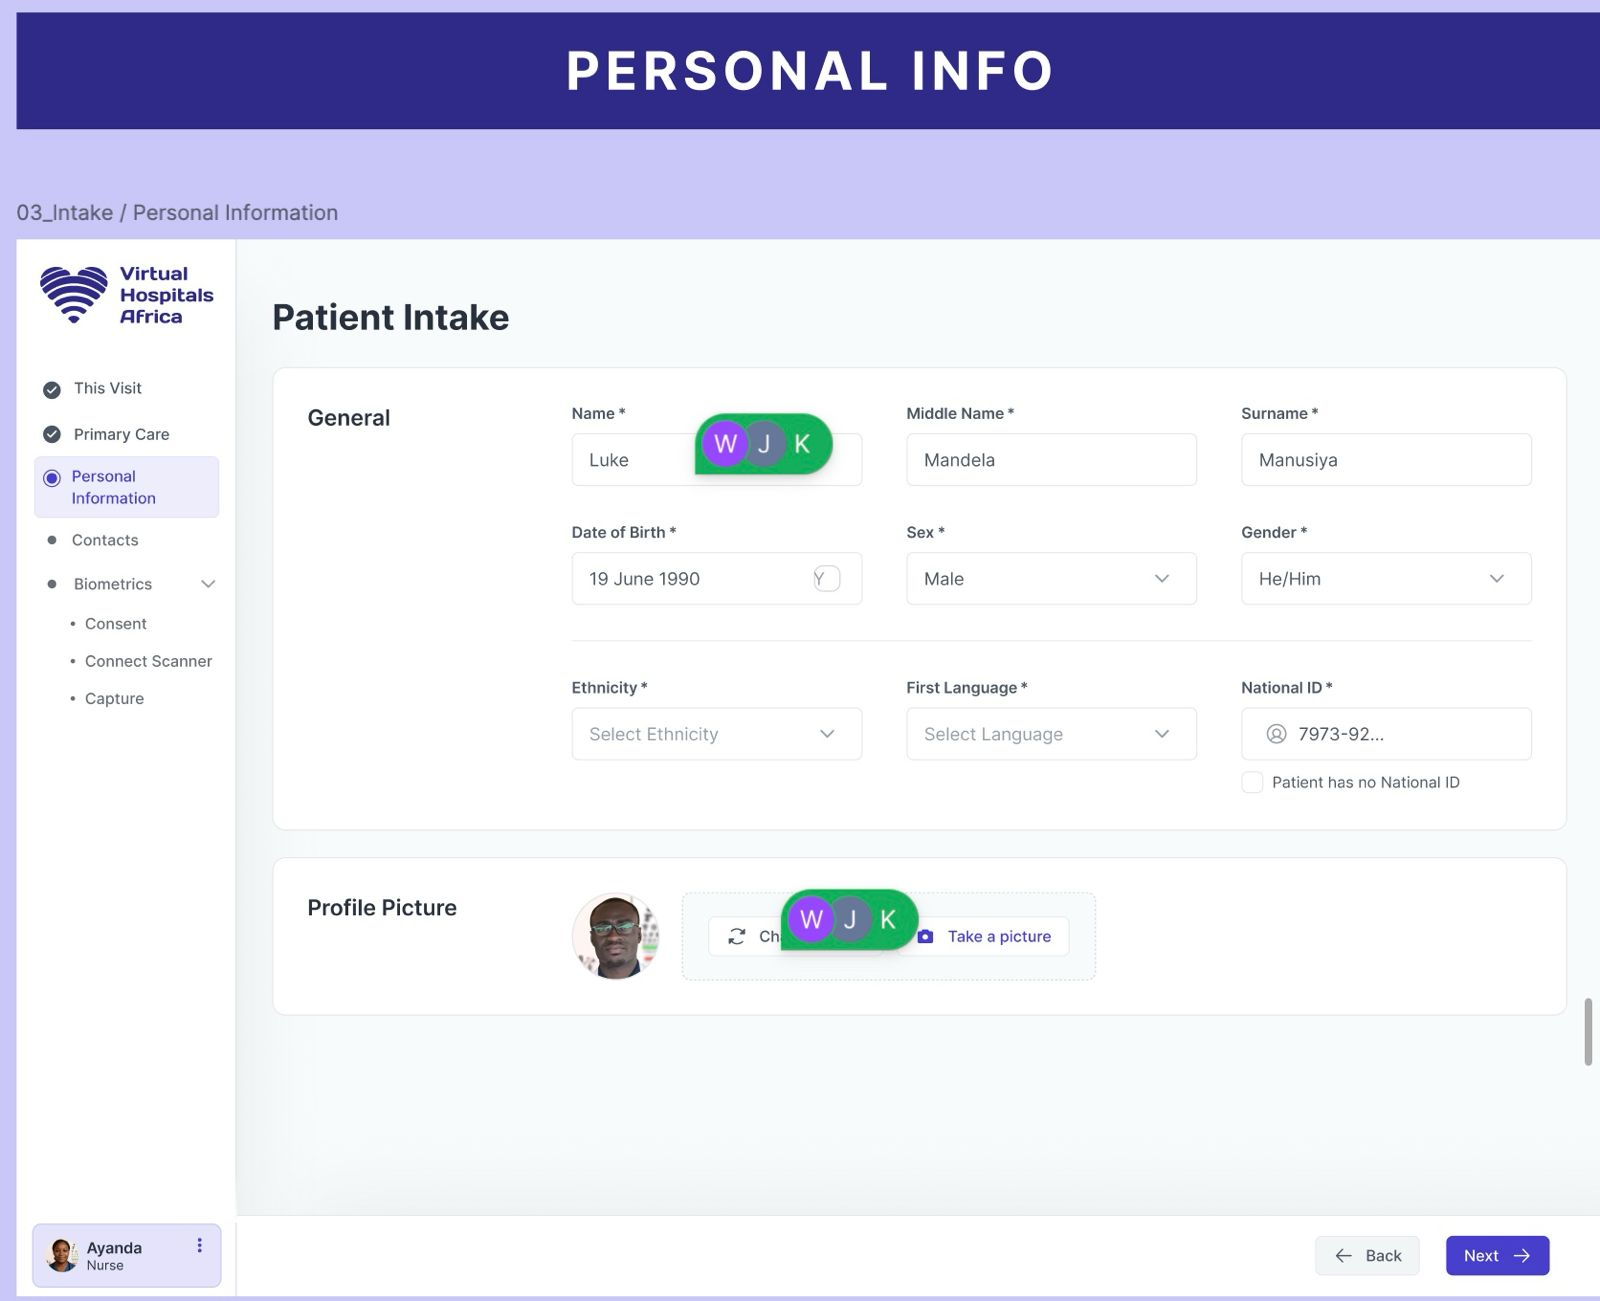
\includegraphics[width=\textwidth]{images/(VHA)-3.jpg}
        \caption{Third version with left-side navigation and unified buttons}
        \label{fig:design-3}
    \end{minipage}\hfill
    \begin{minipage}{0.47\textwidth}
        \centering
        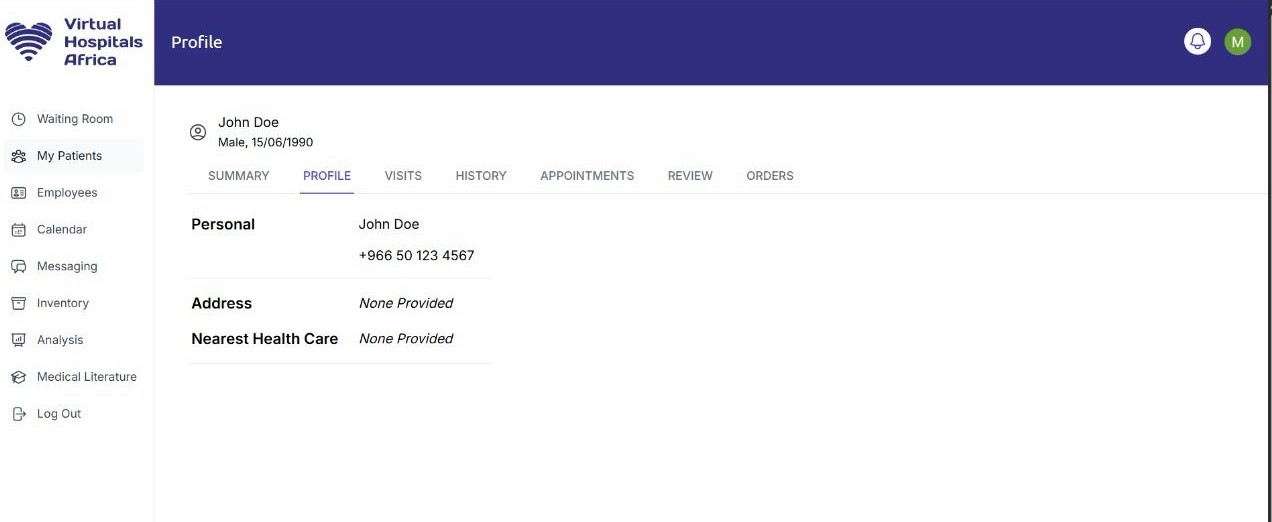
\includegraphics[width=\textwidth]{images/(VHA)-4.jpg}
        \caption{Patient profile page – issues in current interface}
        \label{fig:design-4}
    \end{minipage}
\end{figure}
\begin{figure}[H]
    \centering
    \begin{minipage}{0.47\textwidth}
        \centering
        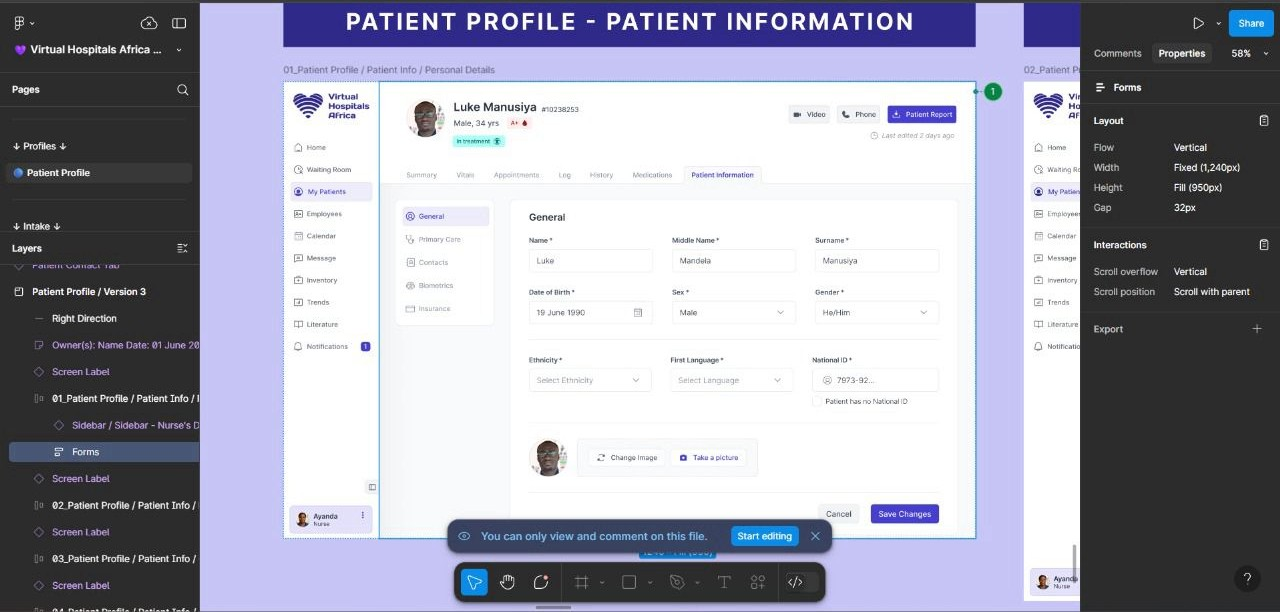
\includegraphics[width=\textwidth]{images/(VHA)-5.jpg}
        \caption{Redesigned patient profile with improved info card and modules}
        \label{fig:design-5}
    \end{minipage}\hfill
    \begin{minipage}{0.47\textwidth}
        \centering
        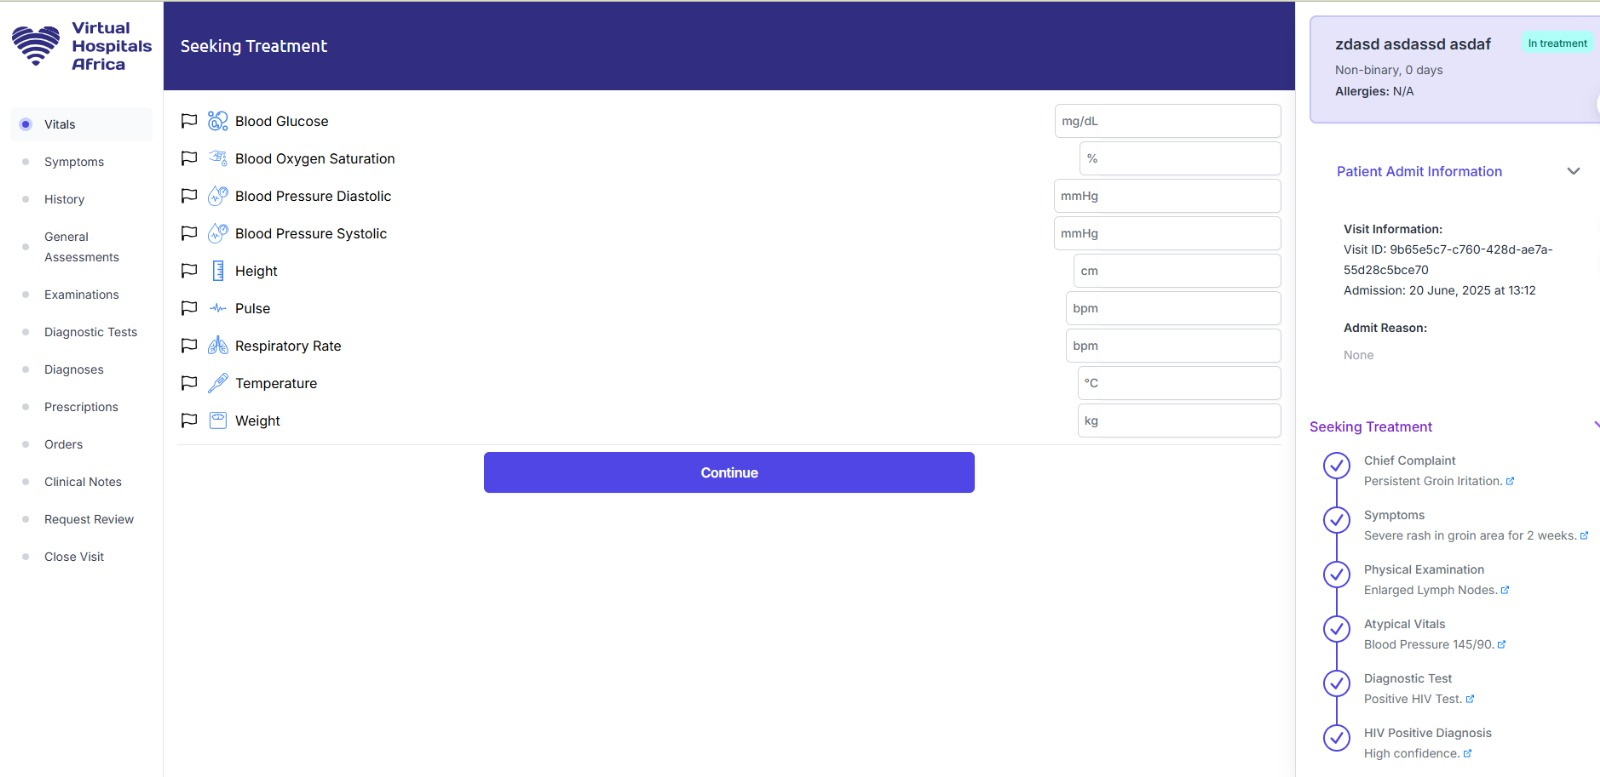
\includegraphics[width=\textwidth]{images/(VHA)-6.jpg}
        \caption{Vitals page – issues in original layout}
        \label{fig:design-6}
    \end{minipage}
\end{figure}
% === END AUTO-INSERTED DESIGN ===


\subsection{Smart Hospital}
\label{subsec:subsec02}

\section{Back-end Design and Implementations}
\label{sec:sec03}
